\documentclass[serif, aspectratio=169]{beamer}
%\documentclass[serif]{beamer}  % for 4:3 ratio

%\RequirePackage{minted2}
\usepackage[T1]{fontenc} 
\usepackage[utf8]{inputenc}
\usepackage{fourier} % see "http://faq.ktug.org/wiki/uploads/MathFonts.pdf" for other options
\usepackage{hyperref}
\usepackage{latexsym,amsmath,xcolor,multicol,booktabs,calligra}
\usepackage{graphicx,pstricks,listings,stackengine}
\usepackage{lipsum}
\usepackage{../../../TEMPLATES/template_style}

%imports customs%
\usepackage{caption}    % for subfigures
\usepackage{subcaption} % for subfigures
\usepackage{ragged2e}
\usepackage{booktabs,makecell}
\usepackage{colortbl}
\usepackage{multirow}
\usepackage{cite}
\usepackage{tcolorbox}
\usepackage[sort,authoryear]{natbib}

\author{Julien Bezançon}

\title{Phraseology}
\subtitle{CM 2~: Fixation, Defixation and Refixation}

\institute{julien.bezancon@univ-lorraine.fr / \url{https://julienbez.github.io}}

\date{}

% defs
\def\cmd#1{\texttt{\color{red}\footnotesize $\backslash$#1}}
\def\env#1{\texttt{\color{blue}\footnotesize #1}}

% set colors
\definecolor{hkustyellow}{RGB}{167, 131, 55}
\definecolor{hkustblue}{RGB}{0, 56, 116}
\definecolor{hkustred}{RGB}{209, 51, 59}

\lstset{
    basicstyle=\ttfamily\small,
    keywordstyle=\bfseries\color{deepblue},
    emphstyle=\ttfamily\color{deepred},    % Custom highlighting style
    stringstyle=\color{deepgreen},
    numbers=left,
    numberstyle=\small\color{halfgray},
    rulesepcolor=\color{red!20!green!20!blue!20},
    frame=shadowbox,
}

\begin{document} %  --- --- --- --- --- --- --- --- --- --- --- --- 

\begin{frame}[noframenumbering,plain]
    \titlepage
    \vspace*{-0.6cm}
    \begin{figure}[htpb]
        \begin{center}
            \hspace{0.3cm}
            
\includegraphics[width=0.7\columnwidth]{../../../IMAGES/loria_idmc.png}
        \end{center}
    \end{figure}
\end{frame}

% \begin{frame}    
%     \tableofcontents[sectionstyle=show,
%     subsectionstyle=show/shaded/hide,
%     subsubsectionstyle=show/shaded/hide]
% \end{frame}

\section{Before we start...}

\begin{exoframe}
    \begin{center}
        \Large
        What did you learn during last lecture ? \\
        Any questions ?
    \end{center}
\end{exoframe}

\begin{frame}{Last Lecture Doggy bag}
    \begin{minipage}{0.45\columnwidth}
        \begin{block}{Multiword Expressions}
            \begin{itemize}
                \item Studied in phraseology
                \item Several components
                \item Somewhat fixed
                \item Somewhat idiomatic
                \item Always conventionalized
            \end{itemize}
        \end{block}
        \begin{block}{MWEs and NLP}
            \begin{itemize}
                \item MWE discovery
                \item MWE identification
            \end{itemize}
        \end{block}
    \end{minipage}
    \hfill
    \begin{minipage}{0.45\columnwidth}
        \begin{figure}
            
\includegraphics[width=0.9\columnwidth]{../../../FIGURES/divers/doggybag.jpg}
        \end{figure}
    \end{minipage}
\end{frame}

\begin{exoframe}
    \begin{center}
        \Large
        Last time, we studied MWEs, the objects of phraseology. \\
        \vspace{10pt}
        Today, we will study the phenomenoms related to these objects.
    \end{center}
\end{exoframe}

\section{Fixation, Defixation, Refixation}

\begin{frame}{The Fixation Phenomenom}
    \begin{block}{\citep{} definition}
        \begin{quote}
            "[Fixation] is a dynamic process that takes root in a language through usage and ultimately establishes sequences of all kinds in the lexicon"\footnote{[Le figement] est processus dynamique qui s'installe dans la langue grâce à l'usage et qui finit par fixer des séquences de toutes sortes dans le lexique} %habler et hummer, 2005
        \end{quote}
    \end{block}
    \vfill
    \begin{block}{What is its purpose ?}
        \begin{itemize}
            \item Helps us structure our speech with pre-fabricated sentences (MWEs)
            \item Allows us to easily memorize and use these sentences
            \item $\Rightarrow$ Acts as a linguistic shortcut 
        \end{itemize}
    \end{block}
    % \vfill
    % \begin{center}
    %     \Large
    %     Instead of thinking "how can i say something", one can use a pre-fabricated sequence to express itself.
    % \end{center}
\end{frame}

\begin{frame}{How Does Fixation Happens ?}
    \begin{figure}
        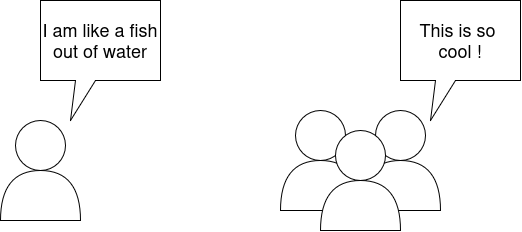
\includegraphics[width=0.9\columnwidth]{../../../FIGURES/phraseology/fixation_BD.png}
        \caption*{Just like that, a new expression was born.}
    \end{figure}
\end{frame}

\begin{frame}{Some Fixation Examples}
    \begin{block}{}
        \begin{itemize}
            \item (En) Killing two birds with one stone
            \item (Fr) Les chats ne font pas des chiens\footnote{Lit. "cats do not raise dogs"}
            \item (Pt) Nem aqui nem na China\footnote{Lit. "not here and not in China"}
        \end{itemize}
    \end{block}
    \vfill
    \begin{center}
        \Large
        Fixation occur in every languages. \\
        Fixation goes with conventionalization.
    \end{center}
\end{frame}

\begin{frame}{One More Fixation Example}
    \begin{block}{Bismillah c'est les ténèbres !\footnote{Bismillah it's darkness !}}
        \begin{figure}
            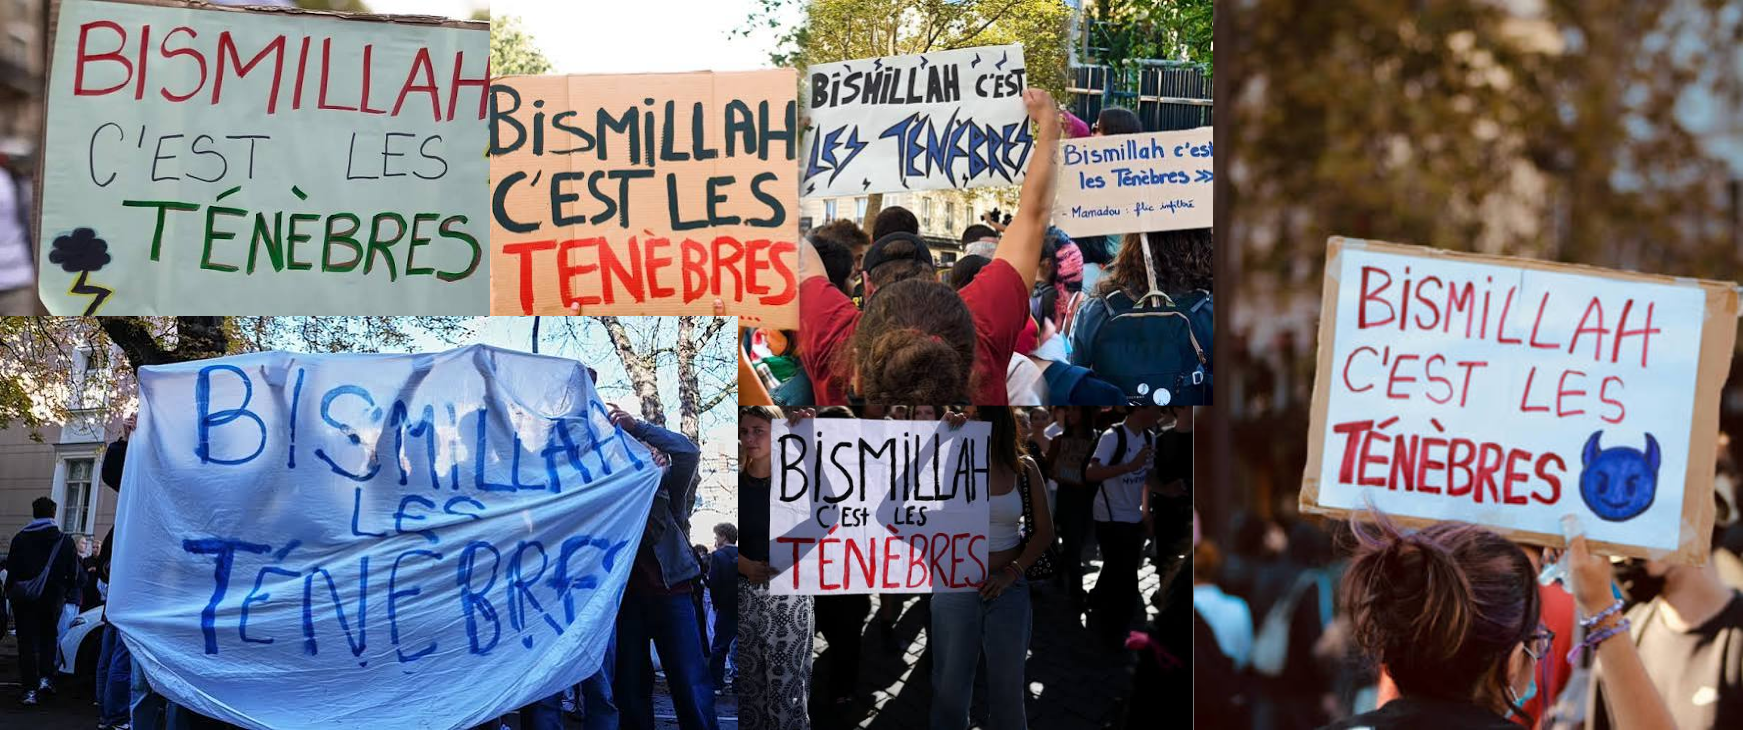
\includegraphics[width=0.8\columnwidth]{../../../FIGURES/phraseology/fixation_bismillah_tenebres.png}
        \end{figure}
    \end{block}
\end{frame}

\begin{frame}{The Defixation Phenomenom}
    \begin{block}{\citep{} definition} %mjeri 2009
        \begin{quote}
            "Any formal or semantical change made on a fixed sequence would be considered as a defixation."\footnote{toute atteinte à la fixité formelle et à la globalité sémantique d'une séquence figée serait considérée comme un défigement}
        \end{quote}
    \end{block}
    \vfill
    \begin{block}{What is its purpose ?}
        \begin{itemize}
            \item Activates the meaning of a MWE + a new meaning
            \item Often used to create satiric / humoristic sentences
            \item $\Rightarrow$ As for fixation, acts as a linguistic shortcut
        \end{itemize}
    \end{block}
\end{frame}

\begin{frame}{How Does Defixation Happens}
    \begin{figure}
        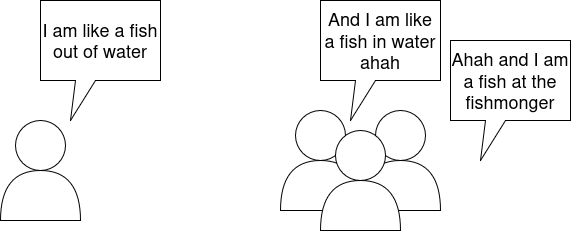
\includegraphics[width=0.9\columnwidth]{../../../FIGURES/phraseology/defixation_BD.png}
        \caption*{We are just playing with an expression, what could happen ?}
    \end{figure}
\end{frame}

\begin{frame}{Some Defixation Examples}
    \begin{block}{}
        \begin{itemize}
            \item Revenge of the Vegans
            \item Lord of the Wings
            \item Requiem for a Drunk
            \item Silence of the Lamborghini
            \item Fifty Shades of Sharks
        \end{itemize}
    \end{block}
    \vfill
    \begin{center}
        \Large
        Fixation is not limited to sayings and locutions. \\
        Pop-culture sentences and citations can become MWEs too.
    \end{center}
\end{frame}

\begin{frame}{More Defixation Examples}
    \begin{block}{Bismillah c'est les ténèbres !\footnote{Bismillah it's darkness !}}
        \begin{figure}
            
\includegraphics[width=0.8\columnwidth]{../../../FIGURES/phraseology/defixation_bismillah_tenebres.png}
        \end{figure}
    \end{block}
\end{frame}

\begin{frame}{The Refixation Phenomenom}
    \begin{block}{\citep{} definition} %bezancon 2025
        \begin{quote}
            "Refixation can be defined as the acceptation of a new form or meaning for a given MWE, which can be more or less close to the original one."\footnote{le refigement peut être défini comme l'acceptation d'une nouvelle forme d'une EMM, plus ou moins éloignée de sa forme originelle.}
        \end{quote}
    \end{block}
    \vfill
    \begin{block}{What is its purpose ?}
        \begin{itemize}
            \item Allows older expression to be relevant again
            \item Acknowledges new entries within a language's lexicon
            \item Can either replace the original MWE or become a new MWE
        \end{itemize}
    \end{block}
\end{frame}

\begin{frame}{How does Refixation Happens ?}
        \begin{figure}
        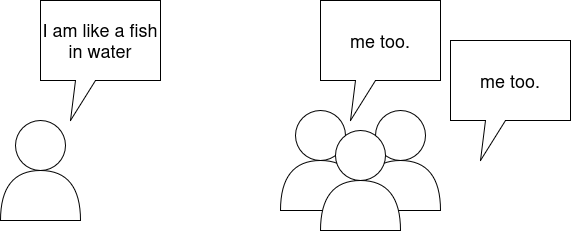
\includegraphics[width=0.9\columnwidth]{../../../FIGURES/phraseology/refixation_BD.png}
        \caption*{Oh no, it's everywhere now !}
    \end{figure}
\end{frame}

\begin{frame}{The Whole Process}
    \begin{figure}
        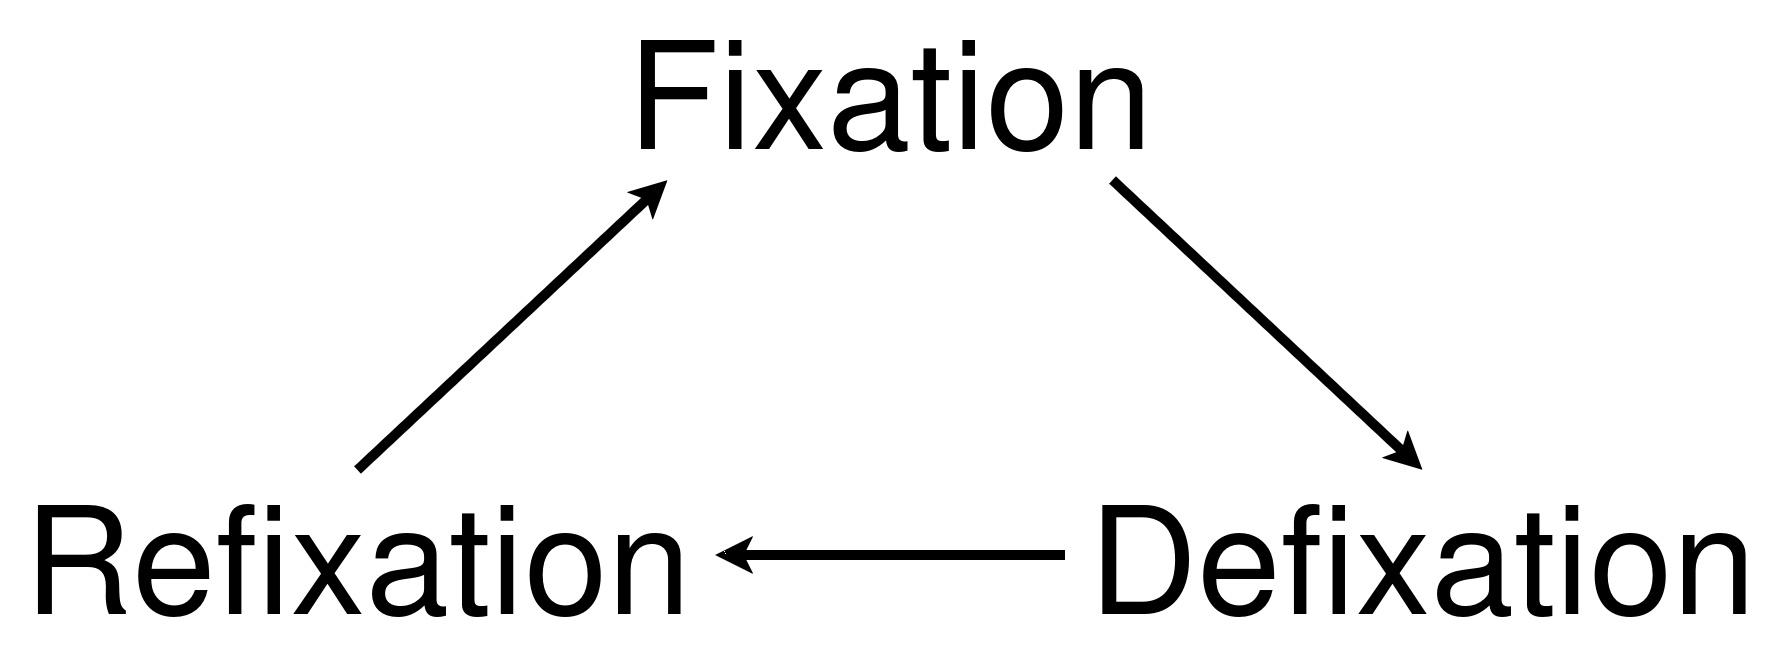
\includegraphics[width=0.8\columnwidth]{../../../FIGURES/phraseology/fixation_circle.png}
    \end{figure}
\end{frame}

\begin{frame}{To Summarize}
    \begin{block}{Fixation - A sequence becomes a MWE}
        \begin{itemize}
            \item To be like a fish out of water
        \end{itemize}
    \end{block}
    \begin{block}{Defixation - A MWE is used to create a variant of itself}
        \begin{itemize}
            \item To be like a fish in the aquarium
            \item To be like a fish at the fishmonger
            \item \textbf{To be like a fish in the water}
        \end{itemize}
    \end{block}
    \begin{block}{Refixation - A MWE variant becomes a MWE}
        \begin{itemize}
            \item To be like a fish in the water
        \end{itemize}
    \end{block}
    \vfill
    \begin{center}
        \Large
        MWEs can undergo this process over and over again.
    \end{center}
\end{frame}

\section{Defixed Multiword Expressions}

\begin{frame}{How to Identify a Defixed MWE ?}
    \begin{block}{Properties}
        \begin{itemize}
            \item Always based on an existing MWE
            \item Caracterized by a formal and/or semantical change
            \item Use their context to add new meaning
            \item Can be recognized by the locutors of a given language 
        \end{itemize}
    \end{block}
    \vfill
    \begin{block}{Examples}
        \begin{itemize}
            \item May the \textbf{Fourth} be with you
            \item It's raining \textbf{nems}
        \end{itemize}
    \end{block}
\end{frame}

\begin{exoframe}{Exercise Time !}
    \begin{block}{Take a look at the following sequences}
        \begin{itemize} \color{white}
            \item Orange is the new pink
            \item Orange is the new grey
            \item Pink is the new black
            \item Gen-z is the new sans-culottes
        \end{itemize}
    \end{block}
    \vfill
    \begin{center}
        \Large
        What do they have in common ? \\
        \pause
        A patern $\Rightarrow$ X is the new Y
    \end{center}
\end{exoframe}

\begin{frame}{Defixed MWEs are hard to Define}%la plupart du temps, c'est de paternes, mais pas que: orange is the old black, pink is not the new black 
% where is the limit ? the current president of the united state is definitly not the new Gandhi
    \begin{block}{Most of the time, defixation follows a patern \citep{}}
        \begin{itemize}
            \item X is the new Y
            \item In space, no one can hear you X
            \item The X, the Y and the Z
        \end{itemize}
    \end{block}
    \vfill
    \begin{block}{But a MWE can be defixed through other means}
        \begin{itemize}
            \item Orange is the old black
            \item Orange is not the new black
            \item The current President of the US is definitely not the new Gandhi
        \end{itemize}
    \end{block}
    \vfill
    \begin{center}
        \Large
        Where is the limit between a defixation and a lambda sequence ?
    \end{center}
\end{frame}

\begin{frame}{How to Deal with Defixed MWEs}
    \begin{center}
        \Large
        Where is the limit between a defixation and a lambda sequence ? \\
        \vspace{10pt}
        We lack both data and analysis !
    \end{center}
    \vfill
    \begin{block}{The current solution}
        \begin{itemize}
            \item \textbf{Step 1:} identify sequences which may correspond to defixed MWEs
            \item \textbf{Step 2:} filter these sequences to only retain defixed MWEs
        \end{itemize}
    \end{block}
\end{frame}

%frame avec typo des transformations
\begin{frame}{Step 1: Typology of Transformations \citep{}} %bezancon 2025
    \begin{figure}
        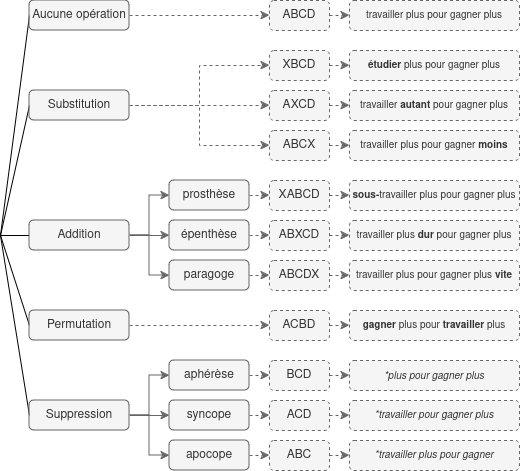
\includegraphics[width=0.5\columnwidth]{../../../FIGURES/phraseology/transformations.png}
    \end{figure}
\end{frame}

\begin{frame}{Step 2: Human Annotation and Dialogue}
    \begin{figure}
        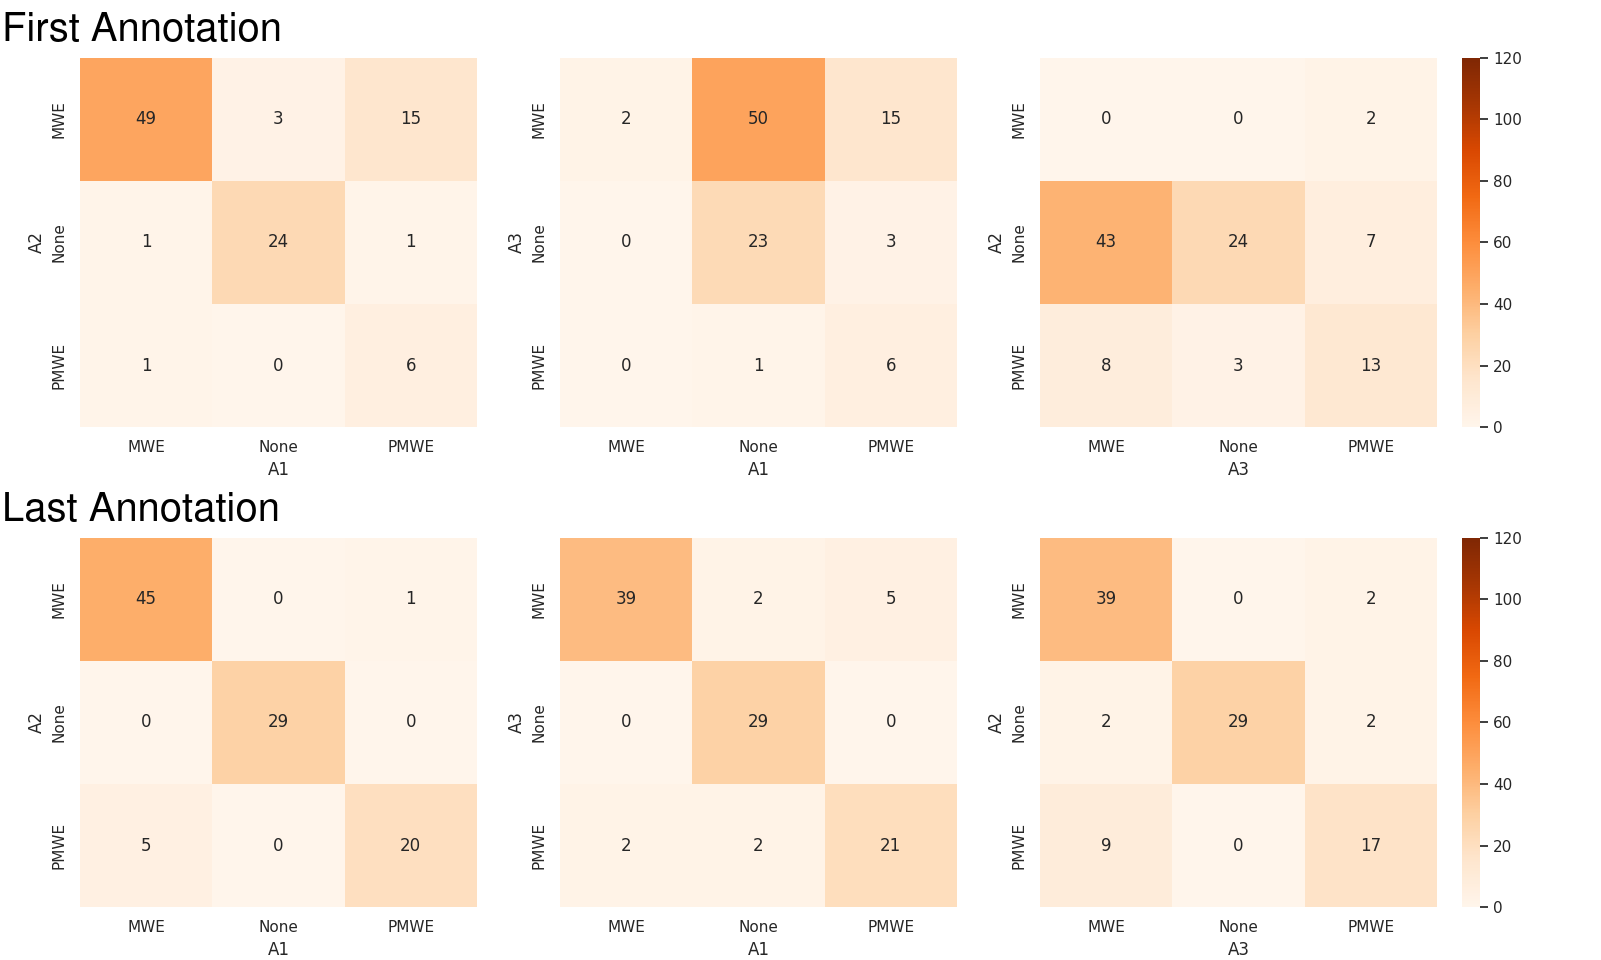
\includegraphics[width=0.8\columnwidth]{../../../FIGURES/phraseology/annotation_matrices_first_last.png}
    \end{figure}
\end{frame}

\begin{frame}{Common Locks and Issues}
    \begin{block}{A lambda sequence is too close to a MWE}
        \begin{itemize}
            \item Ubuntu 26.10 is the new update
            \item j'en peux plus de travailler plus
        \end{itemize}
    \end{block}
    \vfill
    \begin{block}{The defixation is not formal}
        \begin{itemize}
            \item La fin du Monde
            \item Une toile de maître
        \end{itemize}
    \end{block}
    \begin{block}{A defixed MWE is too different from the MWE}
        \begin{itemize}
            \item Trump was not the new Ghandi
        \end{itemize}
    \end{block}
\end{frame}

%demander aux étudiants pk c'est plus dur pour les machines en montrant un défigement et une séquence libre du style : 
%expr de base: travailler plus pour gagner plus
%travailler plus pour gagner moins
%j'en peux plus de travailler autant

%Quiet is the new loud
%Ubuntu 26.10 is the new update for your linux

\section{Defixed Multiword Expressions and NLP}

%exercise together: how to identify PMWEs in texts in NLP
% => faire un schéma au tableau et demander ce qu'il faut en entrée, en sortie, et les règles / méthodes qu'on pourrait utiliser

%idée 1: ASMR => règles, similarité
%idée 2: LSH => machine learning, clustering, paternes

\begin{exoframe}{Exercise Time !}
    \begin{center}
        \Large
        How would you process defixed MWEs in NLP ?
    \end{center}
\end{exoframe}

\begin{frame}{Doggy bag}
    \begin{minipage}{0.45\columnwidth}
        \begin{block}{Linguistic Phenomenoms}
            \begin{itemize}
                \item Fixation
                \item Defixation
                \item Refixation
            \end{itemize}
        \end{block}
        \begin{block}{Defixed MWEs}
            \begin{itemize}
                \item Properties
                \item Locks and issues
                \item How to process them
            \end{itemize}
        \end{block}
    \end{minipage}
    \hfill
    \begin{minipage}{0.45\columnwidth}
        \begin{figure}
            
\includegraphics[width=0.9\columnwidth]{../../../FIGURES/divers/doggybag.jpg}
        \end{figure}
    \end{minipage}
\end{frame}

\end{document}


